\documentclass[12pt,a4paper,oneside]{report}
\usepackage[utf8]{inputenc}
\usepackage[english,russian]{babel}
\usepackage{amsmath}
\usepackage{amssymb}
\usepackage{geometry}
\usepackage{sverb}
\usepackage{graphicx}
\usepackage{pdfpages}

\usepackage{algorithm}
\usepackage{tikz}
\usepackage[noend]{algpseudocode}
\usepackage{titlesec, blindtext, color}
\usepackage{listings}
\usepackage{pgfplots}
\pgfplotsset{compat=newest}
\graphicspath{{../}}
\DeclareGraphicsExtensions{.pdf,.png,.jpg}
\usepackage{tabularx}
\usepackage{subcaption}
\usepackage{colortbl}
\usepackage{multirow}
\usepackage{longtable}
\usepackage{enumitem}
\definecolor{gray75}{gray}{0.75}
\definecolor{Blue}{HTML}{5D8AA8}
\newcommand{\hsp}{\hspace{20pt}}

\newcommand{\RomanNumeralCaps}[1]
{\MakeUppercase{\romannumeral #1}}

% Для листинга кода:
\lstset{ %
	language=c++,                 % выбор языка для подсветки (здесь это С)
	basicstyle=\small\sffamily, % размер и начертание шрифта для подсветки кода
	numbers=left,               % где поставить нумерацию строк (слева\справа)
	numberstyle=\tiny,           % размер шрифта для номеров строк
	stepnumber=1,                   % размер шага между двумя номерами строк
	numbersep=5pt,                % как далеко отстоят номера строк от подсвечиваемого кода
	showspaces=false,            % показывать или нет пробелы специальными отступами
	showstringspaces=false,      % показывать или нет пробелы в строках
	showtabs=false,             % показывать или нет табуляцию в строках
	frame=single,              % рисовать рамку вокруг кода
	tabsize=2,                 % размер табуляции по умолчанию равен 2 пробелам
	captionpos=t,              % позиция заголовка вверху [t] или внизу [b] 
	breaklines=true,           % автоматически переносить строки (да\нет)
	breakatwhitespace=false, % переносить строки только если есть пробел
	escapeinside={\#*}{*)}   % если нужно добавить комментарии в коде
}

%titlefromat определяет стиль заголовка элемента внутри {}
\titleformat{\chapter}[hang]{\Huge\bfseries}{\thechapter.\textcolor{gray75}\hsp}{0pt}{\Huge\bfseries}

\geometry{pdftex, left = 2cm, right = 2cm, top = 2.5cm, bottom = 2.5cm}

\begin{document}
\newcommand{\specchapter}[1]{\chapter*{#1}\addcontentsline{toc}{chapter}{#1}}
\newcommand{\specsection}[1]{\section*{#1}\addcontentsline{toc}{section}{#1}}
\newcommand{\specsubsection}[1]{\subsection*{#1}\addcontentsline{toc}{subsection}{#1}}

% геометрия


\setcounter{tocdepth}{4} % фикс переноса 
\righthyphenmin = 2
\tolerance = 2048


\thispagestyle{empty}

\begin{titlepage}
	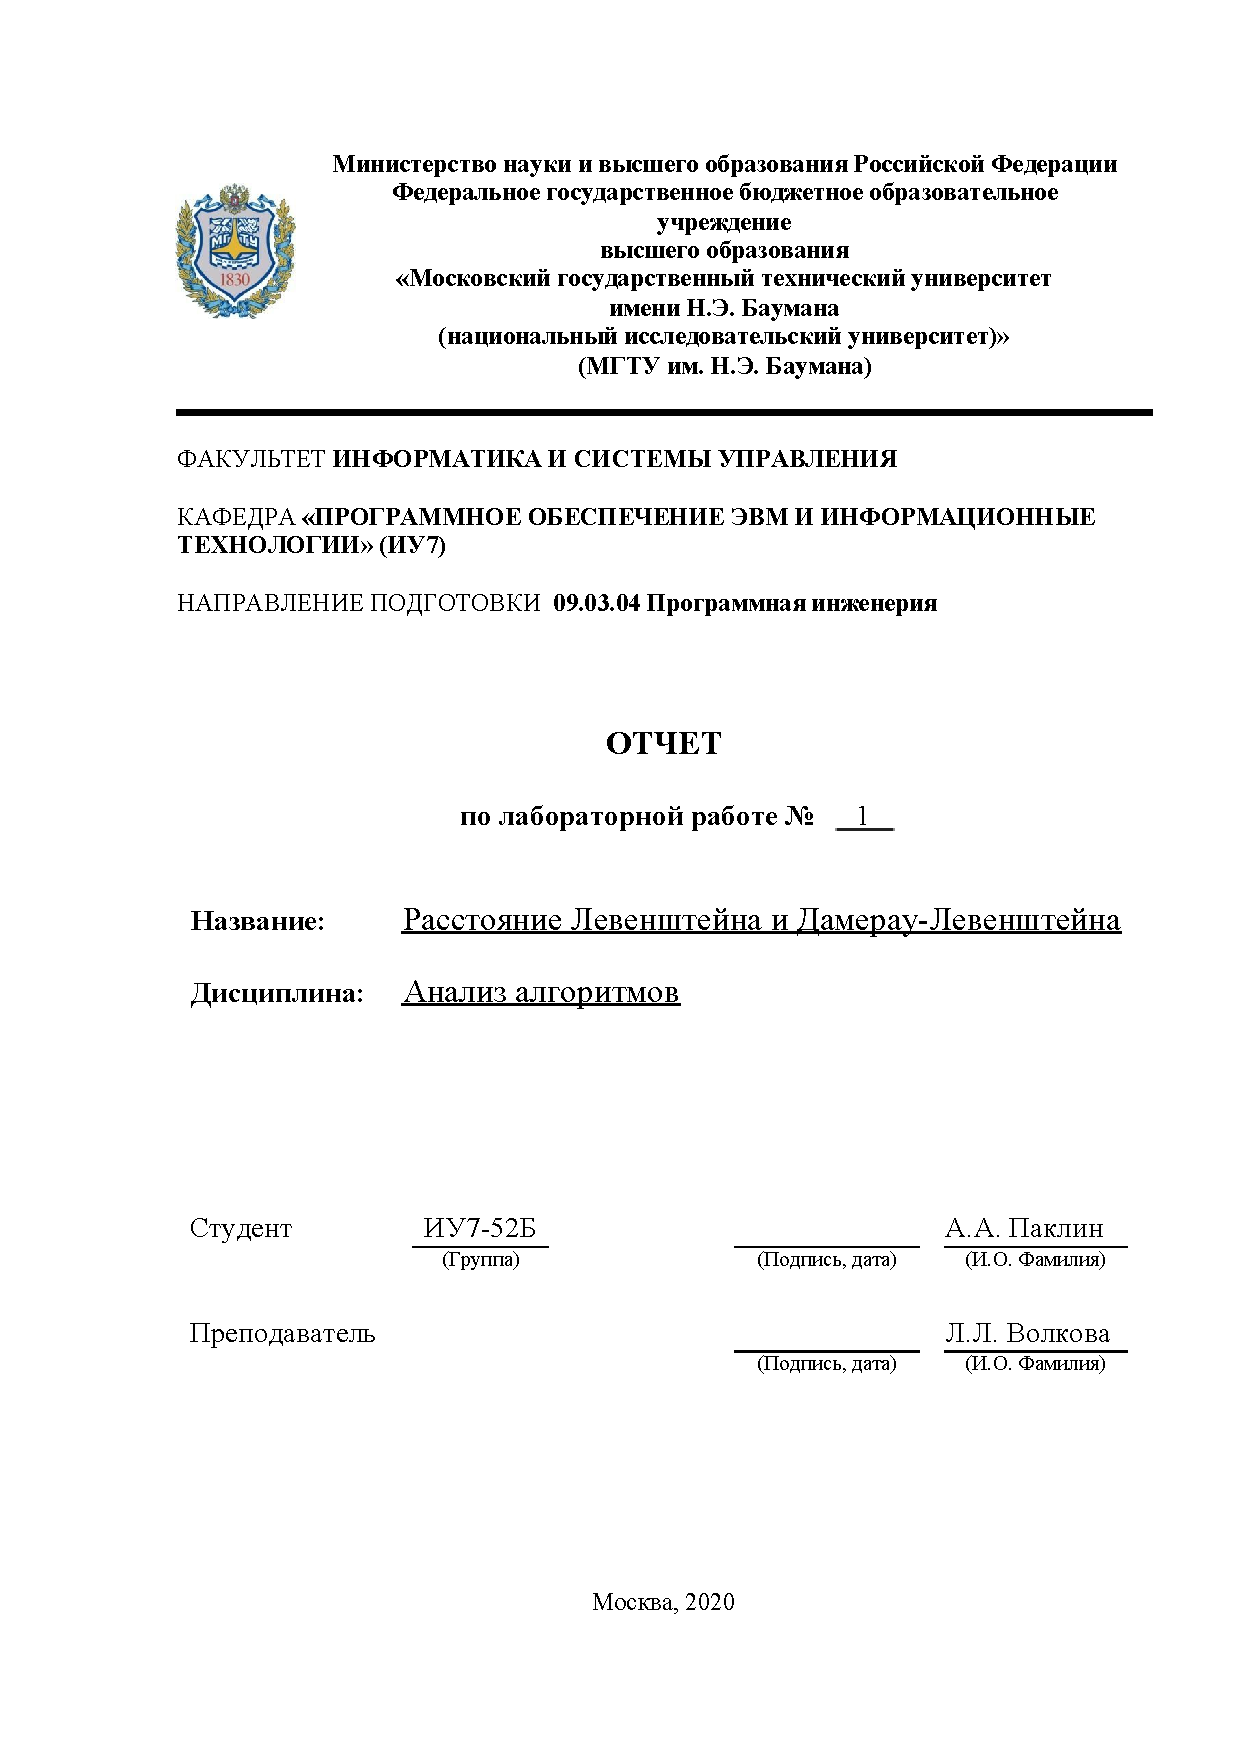
\includepdf[pages=-]{title1.pdf}
\end{titlepage}
\newpage

\renewcommand*\contentsname{Оглавление}
\tableofcontents
\setcounter{page}{1}
\newpage

\makeatletter 
\renewcommand{\figurename}{Рисунок}
\renewcommand{\thefigure}{\@arabic\c@figure}
\makeatother

\setcounter{figure}{0}

\chapter*{Введение}
\addcontentsline{toc}{chapter}{Введение}
\qquad\textbf{Расстояние Левенштейна} - минимальное количество редакторских операций, которое необходимо для превращения одной строки в другую(или другими словами - расстояние между строками).\\

Расстояние Левенштейна используется в следующих сферах:
\begin{itemize}
	\item поисковики - строка поиска Яндекс: автоисправление, автозамена;
	\item бионформатика - в белке каждая молекула представляется буквой из ограниченного алфавита, и белки представляются строками, которые можно сравнивать.
\end{itemize}


Целью данной лабораторной работы является изучение метода динамического программирования на материале алгоритмов
Левенштейна и Дамерау-Левенштейна. \\

Задачами данной лабораторной являются:
\begin{enumerate}
	\item изучение алгоритмов Левенштейна и Дамерау-Левенштейна нахождения расстояния между строками;
	\item применение метода динамического программирования для матричной реализации указанных алгоритмов; 
	\item получение практических навыков реализации указанных алгоритмов: двух алгоритмов в матричной версии и одного из алгоритмов в рекурсивной версии; 
	\item сравнительный анализ линейной и рекурсивной реализаций выбранного алгоритма определения расстояния между строками по затрачиваемым ресурсам (времени и памяти); 
	\item экспериментальное подтверждение различий во временнóй эффективности рекурсивной и
	нерекурсивной реализаций выбранного алгоритма определения расстояния между строками при
	помощи разработанного программного обеспечения на материале замеров процессорного времени
	выполнения реализации на варьирующихся длинах строк; 
	\item описание и обоснование полученных результатов в отчете о выполненной лабораторной
	работе, выполненного как расчётно-пояснительная записка к работе. 
\end{enumerate}

\chapter{Аналитическая часть}
\qquad Задача по нахождению расстояния Левенштейна заключается в поиске минимального количества операций вставки/удаления/замены для превращения одной строки в другую.

При нахождении расстояния Дамерау — Левенштейна добавляется операция транспозиции (перестановки соседних символов).  

Действия обозначаются так:
\begin{enumerate}
	\item D (delete) — удалить;
	\item I (insert) — вставить;
	\item R (replace) — заменить;
	\item M(match) - совпадение.
\end{enumerate}

Пусть $S_{1}$ и $S_{2}$ — две строки (длиной M и N соответственно) над некоторым алфавитом, тогда расстояние Левенштейна можно подсчитать по следующей рекуррентной формуле, описанной в книге \cite{Skieyna}:

\begin{displaymath}
D(i,j) = \left\{ \begin{array}{ll}
0, & \textrm{$i = 0, j = 0$}\\
i, & \textrm{$j = 0, i > 0$}\\
j, & \textrm{$i = 0, j > 0$}\\
min(\\
D(S_1[i],S_2[j-1])+1,& \textrm{$ j > 0 \quad //I$}\\
D(S_1[i-1], S_2[j]) +1, &\textrm{$i > 0 \quad //D$}\\
D(S_1[i-1], S_2[j-1]) + \\

\left[ \begin{array}{ll}
0, & \textrm{если $\quad S1[i] == S2[j], \quad //M$}\\
1, & \textrm{иначе $\quad //R$}
\end{array}\right.\\
)
\end{array} \right.
\end{displaymath}\\

где $min()$ возвращает наименьший из аргументов.
\newpage
Расстояние Дамерау-Левенштейна вычисляется по следующей рекуррентной формуле, описанной в книге \cite{Skieyna}:
\begin{displaymath}
D(i,j) = \left\{ \begin{array}{ll}
0, & \textrm{$i = 0, j = 0$}\\
i, & \textrm{$j = 0, i > 0$}\\
j, & \textrm{$i = 0, j > 0$}\\
min(\\
D(S_1[i],S_2[j-1])+1,& \textrm{$ j > 0 \quad //I$}\\
D(S_1[i-1], S_2[j]) +1, &\textrm{$i > 0 \quad //D$}\\
D(S_1[i-1], S_2[j-1]) + \\

\left[ \begin{array}{ll}
0, & \textrm{если $\quad S1[i] == S2[j], \quad //M$}\\
1, & \textrm{иначе $\quad //R$}\\
\end{array}\right.\\
D(S_1[i - 2], S_2[j - 2]) + 1 & \textrm{если $i = 1, j = 1,
	S_1[i] = S_2[j - 1],
	S_1[i - 1] = S_2[j]$}\\
)
\end{array} \right.
\end{displaymath}
\section*{Вывод}
\qquad Была рассмотрена теоретичсекая часть алгоритмов нахождения минимального редакционного расстояния: Левенштейна и Дамерау-Левенштейна.  Отличие которых — наличие дополнительной операции во втором алгоритме. 
\clearpage


\chapter{Конструкторская часть}
\qquad В данном разделе описываются схемы алгоритмов для нахождения минимального редакционного расстояния.
\section{Разработка алгоритмов}
\qquadНа рисунках 1 - 4 представлены схемы алгоритмов, сделанные на основе теоретического материала, представленного в книге \cite{Gasfild}
\begin{figure}[!htpb]
	\centering
	
	\begin{subfigure}[t]{.4\linewidth}
		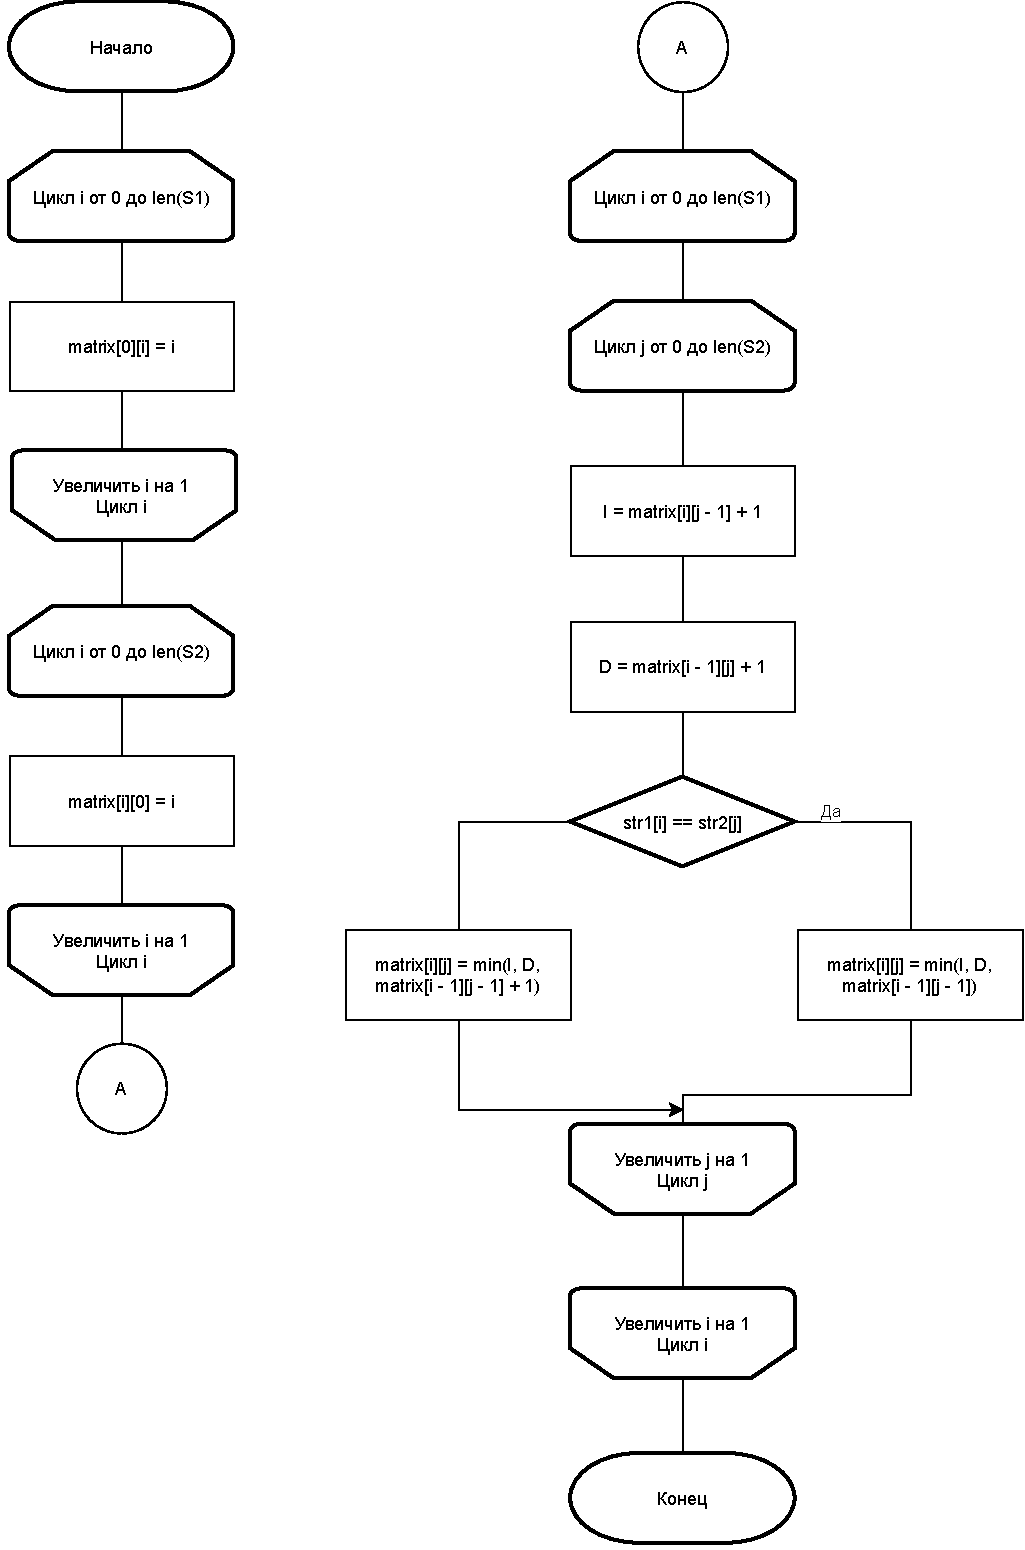
\includegraphics[height=2\linewidth]{matrix_leven}
	\end{subfigure}
	\quad
	
	\caption{Схема матричного алгоритма Левенштейна}
\end{figure}

\begin{figure}[H]
	\centering
	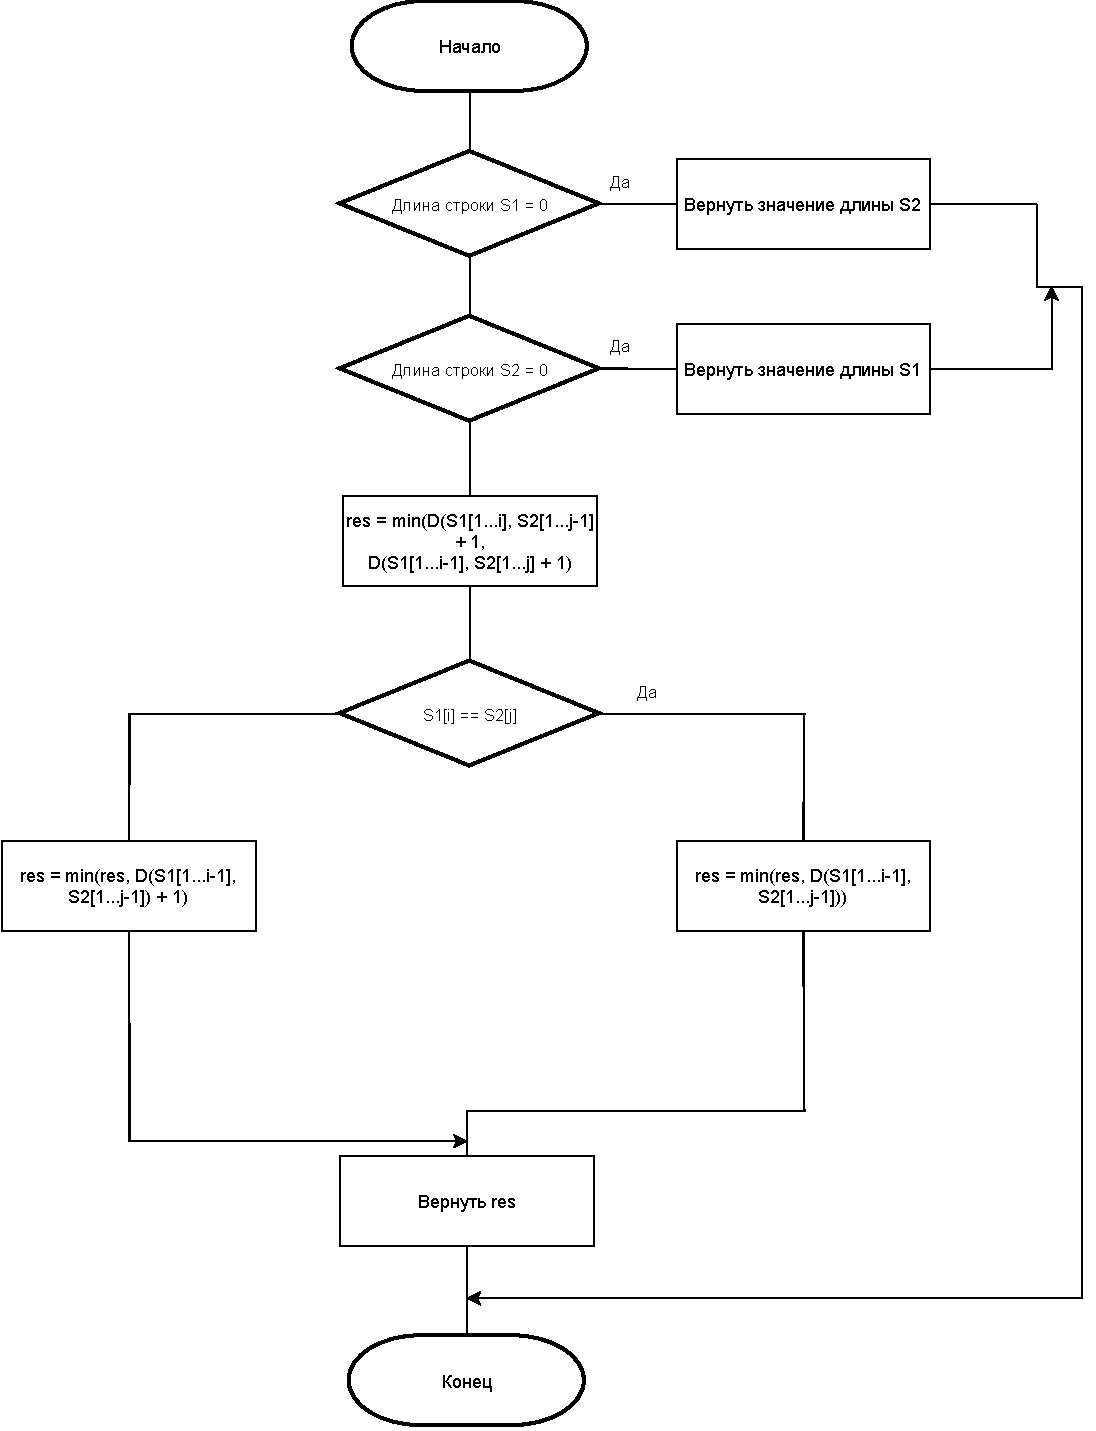
\includegraphics[width=0.8\linewidth]{levenshtein_recursive}
	\caption{Схема рекурсивного алгоритма нахождения расстояния Левенштейна}
\end{figure}

\begin{figure}[H]
	\centering
	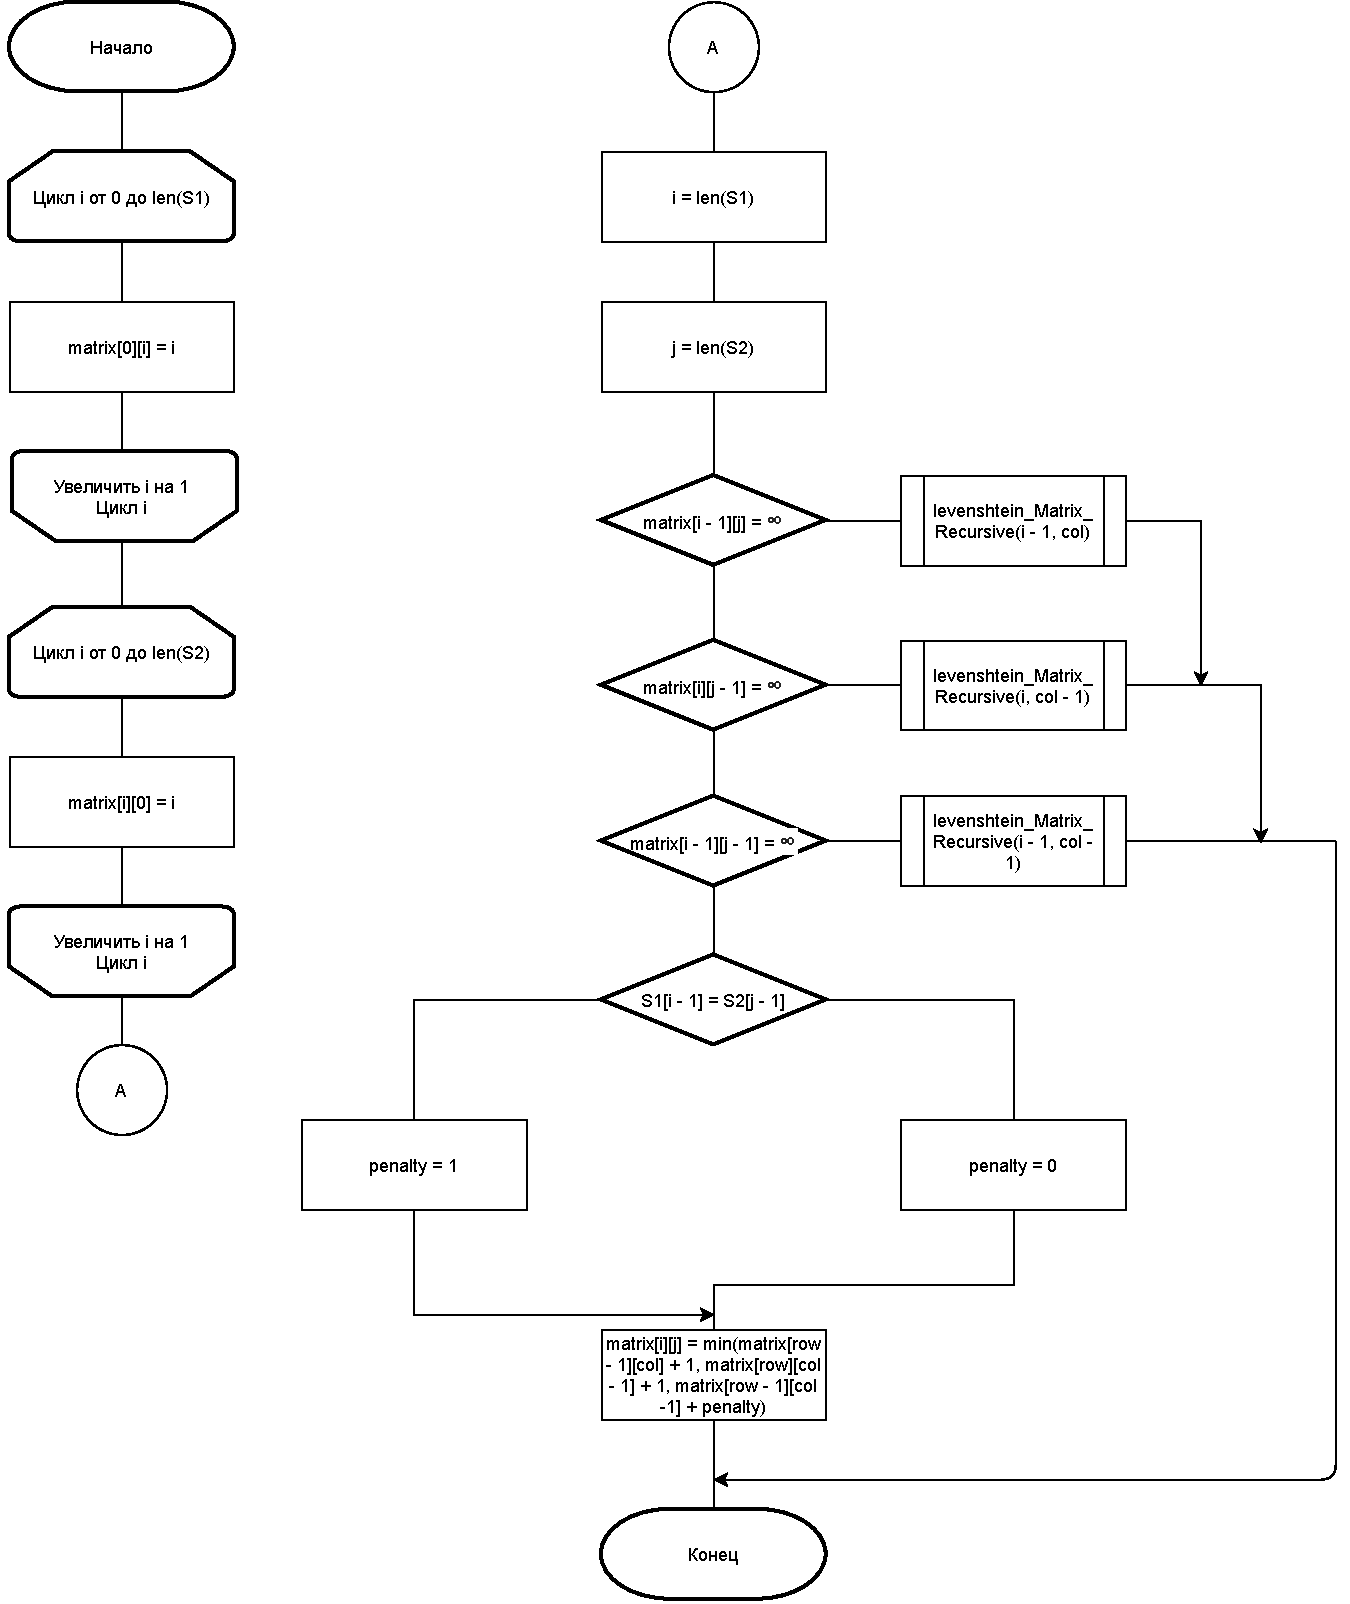
\includegraphics[width=0.8\linewidth]{levenshtein_matrix_recursive}
	\caption{Схема рекурсивного алгоритма нахождения расстояния Левенштейна c заполнением матрицы и дополнительными проверками}
\end{figure}


\begin{figure}[H]
	\centering
	
	\begin{subfigure}[t]{.4\linewidth}
		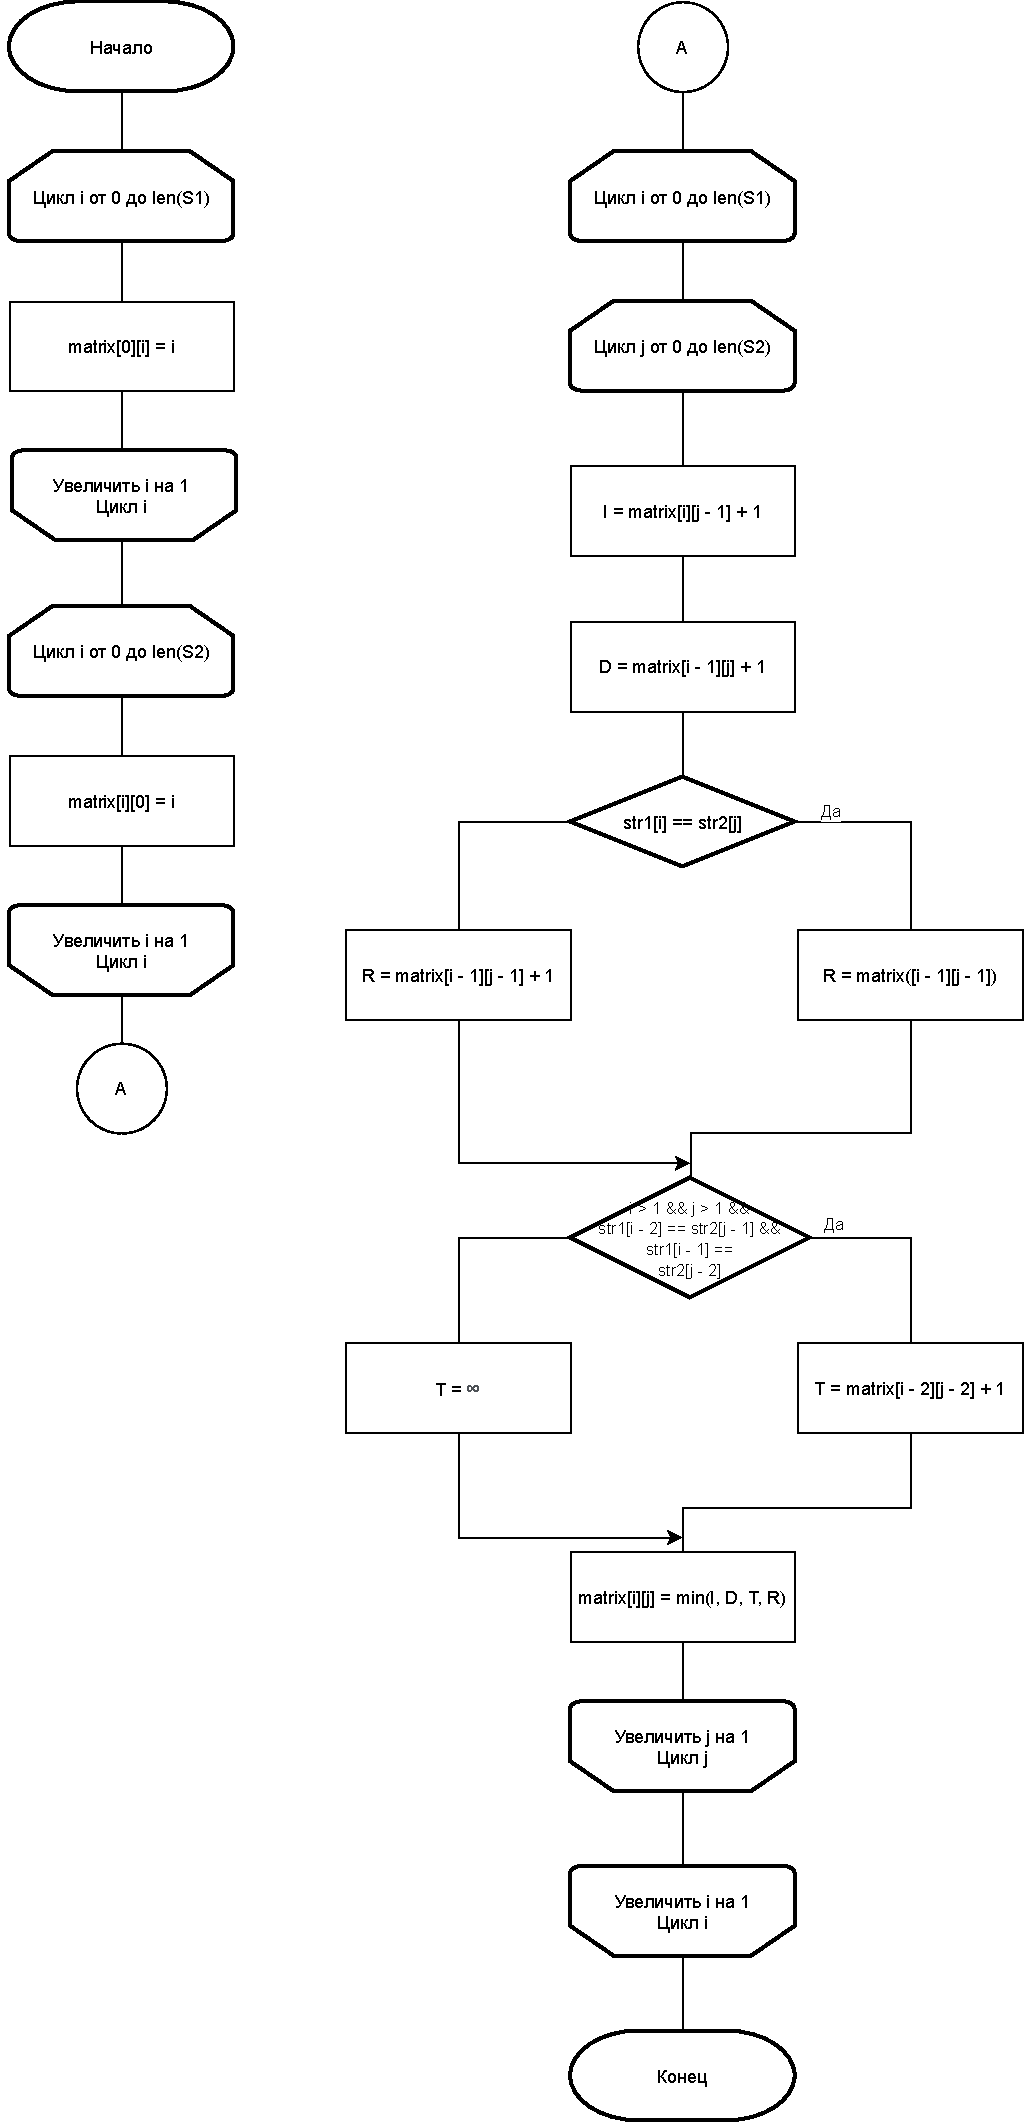
\includegraphics[height=2.3\linewidth, width=1.2\linewidth]{damerau_levenshtein}
	\end{subfigure}
	\quad

	\caption{Схема матричного алгоритма нахождения расстояния Дамерау - Левенштейна}
\end{figure}

\section*{Вывод}
\qquad В данном разделе были проиллюстрированы схемы алгоритмов нахождения минимального редакционного расстояния.


\chapter{Технологическая часть}
\qquad В данном разделе описываются средства реализации,  рассматриваются требования к программному обеспечению, а также приводится реализация алгоритмов на языке C++.
\section{Требования к программному обеспечению}
\qquad \textbf{Требования к вводу:}


\begin{enumerate}
	\item на вход подаются две строки;
	\item буквы в верхнем и нижнем регистрах считаются разными.
\end{enumerate}


\textbf{Требования к программе:}
Две пустые строки - корректный ввод, программа не должна завершаться аварийно.

\section{Средства реализации} 
\qquad Для выполнения лабораторной работы мною был выбран язык C++,  так как он является одним из самых высокопроизводительных языков программирования.
Для замера времени использовалась встроенная библиотека std::chrono\cite{timeit}. 

\newpage
\section{Листинг кода алгоритмов}
\qquad На листинге 3.1 представлена реализация стандартного алгоритма Левенштейна:
\begin{lstlisting}[label=matrix_leven,caption=Функция нахождения расстояния Левенштейна с использованием матрицы]
Matrix<size_t> Levenstein(string_view first, string_view second) {
	auto rows = first.size() + 1;
	auto cols = second.size() + 1;
	Matrix<size_t> result(rows, cols);
	for (size_t i = 0; i < rows; i++) {
		for (size_t j = 0; j < cols; j++) {
			if (i * j == 0) {
				result[i][j] = i | j;
			} else if (first[i - 1] == second[j - 1]) {
				result[i][j] = result[i - 1][j - 1];
			} else {
				result[i][j] = 1 + u_min(
																	result[i - 1][j - 1],
																	result[i][j - 1],
																	result[i - 1][j]
														     );
			}
		}
	}
	return result;
}
\end{lstlisting}

\qquad На листинге 3.2 представлена реализация алгоритма Левенштейна с использованием рекурсии:

\begin{lstlisting}[label=rec_leven,caption=Функция нахождения расстояния Левенштейна с использованием рекурсии]
size_t RecursiveImpl(string_view first, string_view second,
							const size_t i, const size_t j) 
{
	if (i * j == 0) {
		return i | j;
	} else if (first[i - 1] == second[j - 1]) {
		return RecursiveImpl(first, second, i - 1, j - 1);
	}
	return 1 + u_min(
										RecursiveImpl(first, second, i, j - 1),
										RecursiveImpl(first, second, i - 1, j),
										RecursiveImpl(first, second, i - 1, j - 1)
									);
}

size_t RecursiveLevenstein(string_view first, string_view secnd) {
	return RecursiveImpl(first, secnd, first.size() + 1, secnd.size() + 1);
}
\end{lstlisting}

\newpage
\qquad На листинге 3.3 представлена реализация алгоритма Левенштейна с использованием рекурсии и зaполнением матрицы:

\begin{lstlisting}[label=matrx_rec_leven,caption=Функция нахождения расстояния Левенштейна с использованием рекурсии и заполнением матрицы]
size_t RecursiveMatrImpl(Matrix<size_t>& matrix, string_view first,
					string_view second, const size_t i, const size_t j)
{
	if (matrix[i][j] != -1) {
		return matrix[i][j];
	}
	if (i * j == 0) {
		return matrix[i][j] = i | j;
	}
	auto cost = (first[i - 1] != second[j - 1]);
	return matrix[i][j] = cost + u_min(
									RecursiveMatrImpl(matrix, first, second, i, j - 1),
									RecursiveMatrImpl(matrix, first, second, i - 1, j),
									RecursiveMatrImpl(matrix, first, second, i - 1, j - 1)
																	   );
}

Matrix<size_t> RecursiveMatrLevenstein(string_view first, 
																		 	 string_view second) 
{
	Matrix<size_t> result(first.size() + 1, second.size() + 1);
	result.assign(-1);
	RecursiveMatrImpl(result, first, second, first.size(), second.size());
	return result;
}

\end{lstlisting}

\newpage

\qquad На листинге 3.4 представлена реализация стандартного алгоритма Дамерау-Левенштейна:

\begin{lstlisting}[label=matrx_rec_leven,caption=Функция нахождения расстояния Дамерау-Левенштейна с использованием матрицы]
Matrix<size_t> DamerauLevenstein(string_view first, string_view second) {
	auto rows = first.size() + 1;
	auto cols = second.size() + 1;
	Matrix<size_t> result(rows, cols);
	
	for (size_t i = 0; i < rows; i++) {
		for (size_t j = 0; j < cols; j++) {
			if (i * j == 0) {
				result[i][j] = i | j;
			} else if (first[i - 1] == second[j - 1]) {
				result[i][j] = result[i - 1][j - 1];
			} else {
				result[i][j] = 1 + u_min(
																	result[i - 1][j - 1],
																	result[i][j - 1],
																	result[i - 1][j]
															  );
			}
			if (i > 1 && j > 1 && first[i - 1] == second[j - 2]
						&& first[i - 2] == second[j - 1])
			{
					result[i][j] = u_min(
																result[i][j],
																result[i - 2][j - 2] + 1
														  );
			}
		}
	}
	return result;
}
\end{lstlisting}


\section*{Вывод}
\qquad В данном разделе была приведены реализация алгоритмов поиска минимального редакционного расстояния на языке программирования C++.

\chapter{Экспериментальная часть}
\qquad В данном разделе иллюстрируются примеры работы программы, результаты тестирования, а также описывается постановка эксперимента по замеру времени и памяти. 
\section{Тестирование программы}
\qquad Примеры работы для каждой из операций:

\setcounter{figure}{4}
\renewcommand{\thesubfigure}{\arabic{subfigure}}

\begin{figure}[H]
	\centering
	
	\begin{subfigure}[b]{0.3\textwidth}
		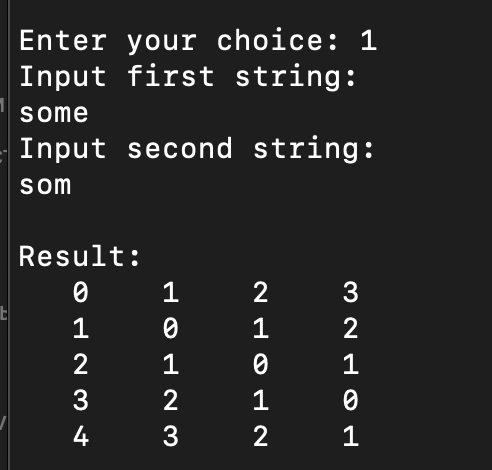
\includegraphics[width=\linewidth]{delete}
		\caption{удаление символов из строки}
	\end{subfigure}
	~
	\begin{subfigure}[b]{0.3\textwidth}
		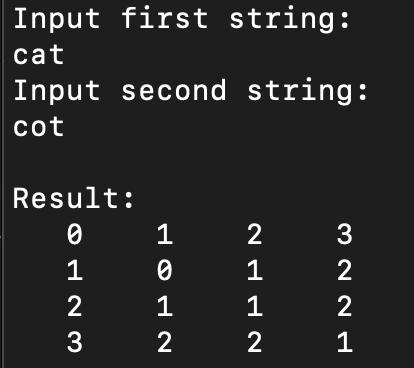
\includegraphics[width=\linewidth]{replace}
		\caption{замена}
	\end{subfigure}
	~
		\begin{subfigure}[b]{0.3\textwidth}
		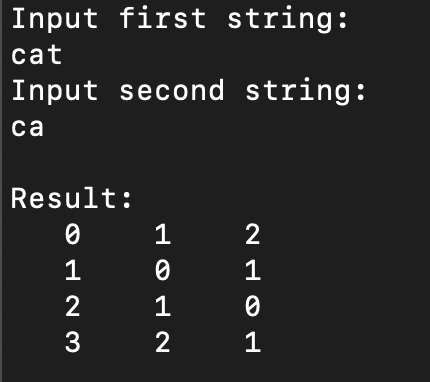
\includegraphics[width=\linewidth]{add}
		\caption{добавление}
	\end{subfigure}
	~
	\begin{subfigure}[b]{0.3\textwidth}
		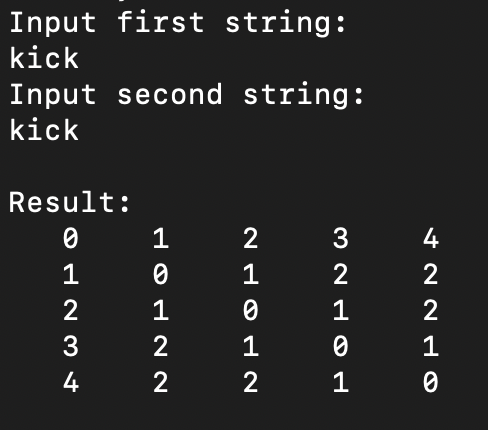
\includegraphics[width=\linewidth]{same}
		\caption{ввод одинаковых строк}
	\end{subfigure}
	~
	\begin{subfigure}[b]{0.3\textwidth}
		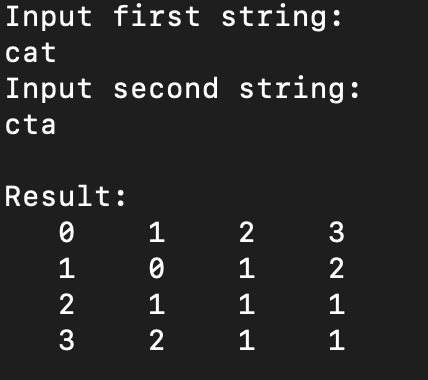
\includegraphics[width=\linewidth]{swap}
		\caption{перестановка}
	\end{subfigure}
	
	\caption{Результаты работы программы}
\end{figure}

\qquad Также было проведено тестирование методом черного ящика, результаты показаны в таблице 4.2:


\setcounter{table}{1}
\newcolumntype{P}[1]{>{\centering\arraybackslash}p{#1}}
\begin{table}[H]
	\centering
	\begin{tabular} {|P{1cm}|P{3cm}|P{3cm}|P{3cm}|P{3cm}|} 
		\hline
		№ & Первое слово & Второе слово &Ожидаемый результат(Левенштейн, Дамерау-Левенштейн) & Полученный результат\\ [0.8ex] 
		\hline\hline
		1 & kot & skat & 2 2& 2 2\\
		\hline
		2 & kate & ktae &2 1 &2 1\\
		\hline
		3 & abacaba & aabcaab& 4 2& 4 2\\
		\hline
		4 & sobaka & sboku& 3 3& 3 3\\
		\hline
		5 & qwerty & queue& 4 4& 4 4\\
		\hline
		6 & apple & aplpe& 2 1& 2 1\\
		\hline
		7 & bmstu & utsmb& 4 4& 4 4\\
		\hline
	\end{tabular}
	\caption{Таблица результатов тестов}
\end{table}

\section{Постановка эксперимента по замеру времени и памяти}
\qquad В рамках данной лабораторной работы были проведены слудующие эксперименты:
\begin{enumerate}
	\item теоретический замер потребляемой памяти всеми четырьмя алгоритмами на строках длины 10;
	\item сравнение скорости работы матричных алгоритмов Левенштейна и Дамерау-Левенштейна на строках длиной от 1000 до 2000 включительно. Один эксперимент проводился 50 раз;
	\item сравнение скорости работы рекурсивного алгоритма Левенштейна и рекурсивного алгоритма Левнештейна с матрицей на строках длиной от 1 до 12 включительно. Один эксперимент ставился 5 раз;
	\item сравнение трех алгоритмов Левенштейна на строках длиной от 1 до 12 включительно. Один эксперимен проводился 5 раз.
\end{enumerate}
\newpage
\section{Сравнительный анализ на материале экспериментальных данных}

\qquad В таблице 4.3 представлен список основных сущностей, используемых в алгоритмах, и количество памяти, которое занимает каждая из них. 


\begin{table}[H]
	\centering
	\begin{tabular}{|p{3cm}|p{10cm}|p{3cm}|} 
		\hline
	 Сущность & Описание                                                                                                                                                                                                                                                  & Размер(64 битная архитектура) в байтах  \\ 
		\hline
		Целое число                                & Машинно зависимая величина.                                                                                                                                                                           & 4                             \\ 
		\hline
		Массив рун                                 & Руна - это псевдоним для целого беззнакового 32 битного числа~                                                                                                                                                                                            & len(arr) * 4                  \\ 
		\hline
		Вектор / Строка                                       & Данная сущность по сути представляет собой динамический массив. & 24                             \\ 
		\hline
		Ссылка                                  &  Объект, указывающий на определенные данные, но не хранящий их.                                                                                                   & 4                             \\
		\hline
	\end{tabular}
	\caption{Память, занимаемая различными сущностями в C++}
\end{table}

\qquad В таблице 4.4 видно, что потребляемая память у рекурсивных алгоритмов зависит от максимальной глубины рекурсии, которая равна максимальной длине из двух слов. 
\begin{longtable}[H]{|p{3cm}|p{3cm}|p{5cm}|p{5cm}|}
	\hline
 Алгоритм & Используемые сущности                                      & Память, занимаемая каждой сущностью(в байтах) & Потребляемая память для всего алгоритма(64 битная архитектура)                          \\
	\hline
	\multirow{4}{3cm}{Матричный Левенштейн}                                                                                                                                                                    & Две строки                                 & len(s1) * 2 + len(s2) * 2   + 48                & \multirow{4}{5cm}{2 * (len(s1) + len(s2)) + 88 + (len(s1) + 1)*(24 + (len(s2) + 1)* 4)}  \\ 
	\cline{2-3}
	& Вектор векторов для представления матрицы&  (len(s1) + 1)*(24 + (len(s2) + 1)* 4)              + 24                             &                                                                                         \\ 
	\cline{2-3}
	& Четыре переменные типа size\_t для итерации в цикле и хранения длины строк               & 16                                            &                                                                                         \\ 
	\cline{2-3}

	\hline
	\multirow{4}{3cm}{Рекурсивный Левенштейн}                                                                                                                                                                  & Две строки                                 & len(s1) * 2 + len(s2) * 2   + 48                    & \multirow{4}{5cm}{(2 * (len(s1) + len(s2)) + 48 + 68 * (макс.уровень рекурсии)}                                          \\ 
	\cline{2-3}
	& Две переменные типа size\_t   для индексации строк                    & 8                                            &                                                                                         \\ 
	\cline{2-3}
	& Указатель для адреса возврата                              & 8                                             &                                                                                         \\ 
	\cline{2-3}
	& Переменная типа size\_t  для ответа                             & 4                                              &                                                                                         \\ 
	\hline
	\multirow{6}{3cm}{Рекурсивный Левенштейн с Матрицей}                                                                                                                                                       & Две строки                                  & len(s1) * 2 + len(s2) * 2  + 48                & \multirow{6}{5cm}{(2 *(len(s1) + len(s2)) + 68 * (макс.уровень рекурсии) + (len(s1) + 1)*(24 + (len(s2) + 1)* 4) + 72 }   \\ 
	\cline{2-3}
	& Вектор векторов для представления матрицы&  (len(s1) + 1)*(24 + (len(s2) + 1)* 4)              + 24                             &                                                                                         \\ 
	\cline{2-3}
	& Две переменные типа size\_t   для индексации строк                  & 8                                            &                                                                                         \\ 
	\cline{2-3}
	& Указатель для адреса возврата                              & 8                                             &                                                                                         \\ 
	\cline{2-3}
	& Переменная типа size\_t  для ответа                             & 4                                             &                                                                                         \\ 
	\cline{2-3}

	\hline
	\multirow{4}{3cm}{Матричный Дамерау-Левенштейн}                                                                                                                                                            & Две строки                                 & len(s1) * 2 + len(s2) * 2   + 48                    & \multirow{4}{5cm}{2 * (len(s1) + len(s2)) + 88 + (len(s1) + 1)*(24 + (len(s2) + 1)* 4)}                                         \\ 
	\cline{2-3}
	& Вектор векторов для представления матрицы&  (len(s1) + 1)*(24 + (len(s2) + 1)* 4)              + 24                             &                                                                                         \\ 
	\cline{2-3}
	& Четыре переменные типа size\_t для итерации в цикле и хранения длины строк               & 16                                            &                                                                                         \\ 
	\cline{2-3}
	\hline
	\caption{Теоретическая оценка памяти, потребляемой алгоритмами}
\end{longtable}

\qquad В таблице 4.5 видно, что рекурсивный алгоритм Левенштейна наименее затратный  по памяти. Самым затратным же алгоритмом является рекурсивный Левенштейн с заполнением матрицы, так как помимо потворного вызова рекурсивной функции, в самом начале также аллоцируется память под матрицу, которая в итоге и  заполняется.

\begin{table}[H]
	\centering
	\begin{tabular}{|p{5cm}|p{5cm}|} 
		\hline
Алгоритм & Теоретическое потребление памяти при len(s1) = len(s2) = 10  \\ 
		\hline
		Матричный Левенштейн                       & 876                                                         \\ 
		\hline
		Рекурсивный Левенштейн                     & 768                                                         \\ 
		\hline
		Рекурсивный Левенштейн с матрицей          & 1540                                                         \\ 
		\hline
		Матричный Дамерау Левенштейн               & 876                                                         \\
		\hline
	\end{tabular}
	\caption{Теоретическое потребление памяти алгоритмами при строках длины 10}
\end{table}


\qquad Взглянув на рисунок 6 можно сделать вывод, что матричный алгоритм Дамерау-Левенштейна работает медленнее матричного алгоритма Левенштейна, в силу того, что в Дамерау на каждой итерации цикла нам нужно дополнительно проверять на истинность еще одно условие и в случае прохождения проверки производить дополнительные вычисления.



\qquad В силу того, что рекурсивный алгоритм работает достаточно медленно, график скорости работы двух рекурсивных алгоритмов был разбит на 2 рисунка. Сравнив рисунки 7 и 8 можно сделать вывод, что несмотря на то, что рекурсивный алгоритм Левенштейна с заполнением матрицы требует больше памяти, чем рекурсивный алгоритм без нее, благодаря использованию матрицы он значительно выигрываем в скорости, так как в ходе выполнения не происходит лишних вызовов на повторное вычисление значений, вместо этого они сразу берутся из матрицы.

\qquad Взглянув на рисунок 6 можно сделать вывод, что матричный алгоритм Дамерау-Левенштейна работает медленнее матричного алгоритма Левенштейна, в силу того, что в Дамерау на каждой итерации цикла нам нужно дополнительно проверять на истинность еще одно условие и в случае прохождения проверки производить дополнительные вычисления.

\begin{figure}[h!]
	\centering
	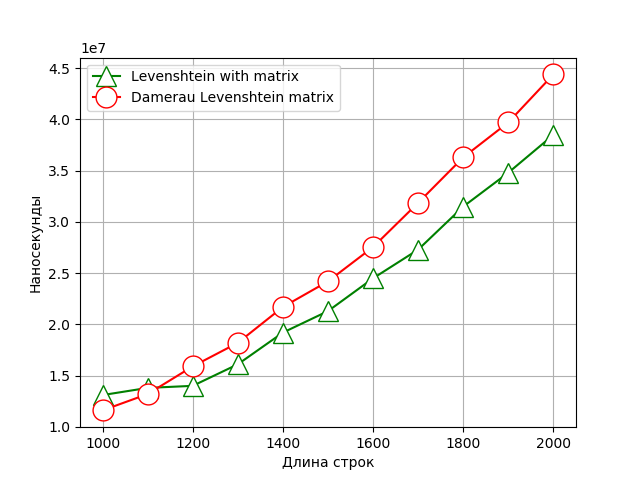
\includegraphics[width=0.54\linewidth]{matrix.png}
	\caption{График работы матричных алгоритмов Левенштейна и Дамерау Левенштейна }
\end{figure}

\qquad В силу того, что рекурсивный алгоритм работает достаточно медленно, график скорости работы двух рекурсивных алгоритмов был разбит на 2 рисунка. Сравнив рисунки 7 и 8 можно сделать вывод, что несмотря на то, что рекурсивный алгоритм Левенштейна с заполнением матрицы требует больше памяти, чем рекурсивный алгоритм без нее, благодаря использованию матрицы он значительно выигрываем в скорости, так как в ходе выполнения не происходит лишних вызовов на повторное вычисление значений, вместо этого они сразу берутся из матрицы.

\begin{figure}[H]
	\centering
	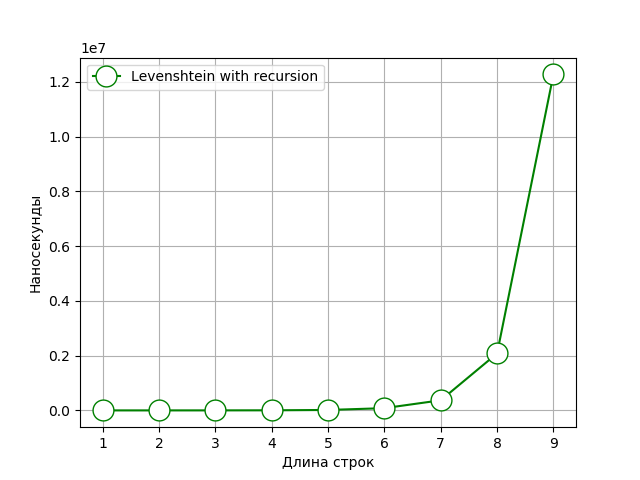
\includegraphics[width=0.54\linewidth]{only_rec.png}
	\caption{График работы рекурсивного алгоритма Левенштейна}
\end{figure}

\begin{figure}[H]
	\centering
	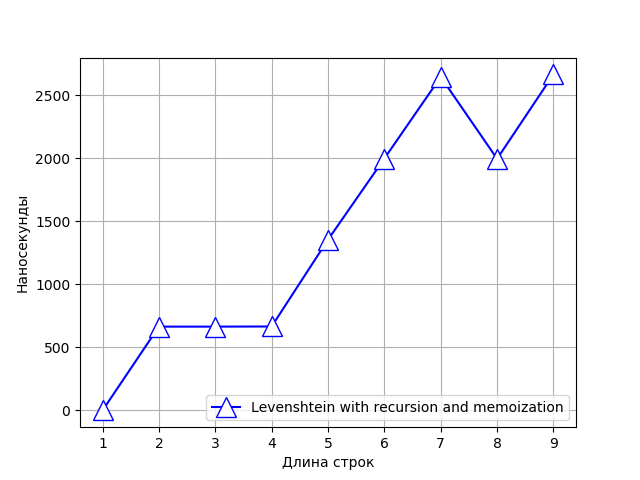
\includegraphics[width=0.54\linewidth]{recM.png}
	\caption{График работы рекурсивного алгоритма с заполнением матрицы Левенштейна}
\end{figure}

\qquad Сравнив рисунок 8 и рисунок 9 можно сделать вывод, что из трех алгоритмов Левенштейна самым медленным оказывается рекурсивный алгоритм, причем при увеличении длины слов появляется проблема того, что результат не может быть получен за приемлимое время. Однако как видно на рисунке 9 добавление матрицы существенно сокращает время выполнения.

\begin{figure}[H]
	\centering
	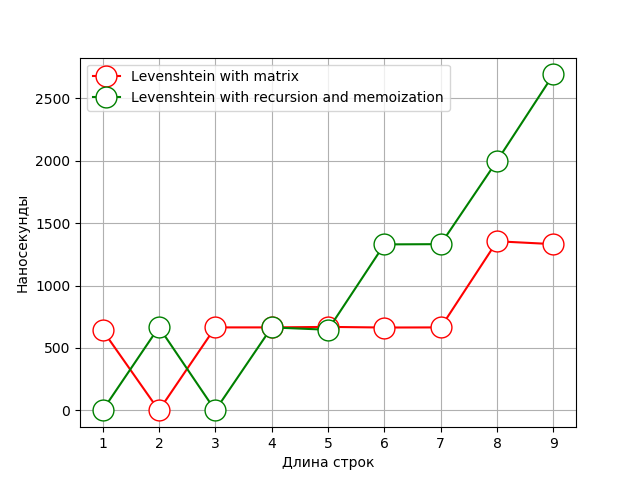
\includegraphics[width=0.54\linewidth]{levs.png}
	\caption{График работы алгоритмов Левенштейна}
\end{figure}

\section*{Вывод} 
\qquad В данном разделе были продемонстрированы результаты экспериментов и сделаны выводы в соответствии с анализом их результатов. Было установлено, что рекурсивный алгоритм работает медленнее остальных, но требует меньше памяти. Самым быстрым алгоритмом оказался матричный Левенштейн.
\chapter*{Заключение}
\qquad В ходе выполнения лабораторной работы были выполнены следующие задачи:
\begin{enumerate}
	\item изучил алгоритмы Левенштейна и Дамерау-Левенштейна нахождения расстояния между строками;
	\item примененил метод динамического программирования для матричной реализации указанных алгоритмов; 
	\item получил практические навыкы реализации указанных алгоритмов: двух алгоритмов в матричной версии и одного из алгоритмов в рекурсивной версии; 
	\item провел сравнительный анализ линейной и рекурсивной реализаций выбранного алгоритма определения расстояния между строками по затрачиваемым ресурсам (времени и памяти); 
	\item экспериментально подтвердил различия во временнóй эффективности рекурсивной и
	нерекурсивной реализаций выбранного алгоритма определения расстояния между строками при
	помощи разработанного программного обеспечения на материале замеров процессорного времени
	выполнения реализации на варьирующихся длинах строк; 
	\item описал и обосновал полученные результаты в отчете о выполненной лабораторной
	работе, выполненного как расчётно-пояснительная записка к работе. 
\end{enumerate}




\newpage


\addcontentsline{toc}{chapter}{Список использованной литературы}
   	\renewcommand{\bibname}{Список использованной литературы}
\begin{thebibliography}{3}
	
	\bibitem{Skieyna}
	Скиена Стивен. Алгоритмы.Руководство к разработке. -- М.:БХВ--Петербруг, 2018. --720 с.
	\bibitem{Gasfild}
	Дэн Гасфилд. Строки, деревья и последовательности в алгоритмах. -- М.:БХВ--Петербруг, 2003. -- 654 с.
			\bibitem{python}Справка по C++ // cppreference URL: https://en.cppreference.com/w/ (дата обращения: 06.10.2020).
	
	\bibitem{timeit} Библиотека для замера времени std::chrono // cppreference URL: https://en.cppreference.com/w/cpp/header/chrono (дата обращения: 06.10.2020)

\end{thebibliography}




\end{document}



